\documentclass[11pt,a4paper]{article}
\usepackage[T1]{fontenc}\usepackage{lmodern}
\usepackage[margin=22mm,headheight=14pt]{geometry}
\usepackage{amsmath,amssymb,bm,booktabs,tabularx,array,graphicx,float,fancyhdr,microtype,xcolor}
\usepackage[colorlinks=true,linkcolor=blue!45!black,urlcolor=blue!45!black,citecolor=blue!45!black]{hyperref}
\setlength{\parindent}{0pt}\setlength{\parskip}{5pt}\renewcommand{\arraystretch}{1.15}
\pagestyle{fancy}\fancyhf{}\fancyhead[L]{\small QFT Project B | Step 8}\fancyhead[R]{\small Group B}\fancyfoot[C]{\thepage}
\newcommand{\dd}{\mathrm{d}}
\begin{document}\hypersetup{pageanchor=false}
\begin{titlepage}\centering\vspace*{3mm}

\includegraphics[width=36mm]{assets/bits_logo.png}\par\vspace{13mm}
{\Large\bfseries BITS PILANI K.K. BIRLA GOA CAMPUS\par}\vspace{3mm}
{\large\bfseries Department of Physics\par}\vspace{18mm}
{\LARGE\bfseries What Quantum Trace Can\\[2mm] a Heavy Particle Leave?\par}\vspace{6mm}
{\large Curvature--Spectator Entanglement\\and the Cosmological Collider\par}\vspace{10mm}
{\large\bfseries Step 8: Convergence and Error Control\par}\vspace{17mm}
{\Large\bfseries Group-B\par}\vspace{5mm}
\begin{tabular}{ll}Priyansh Rawat & 2023B5A70968G\\Mayank Sinha & 2023B5A70942G\\Samarth Bhatnagar & 2023B5A70853G\end{tabular}
\vfill{\large Under Professor: Rudranil Basu\par}\vspace{7mm}{29 October 2026\par}
\end{titlepage}\setcounter{page}{1}\hypersetup{pageanchor=true}
\section{Why the finite starting state matters}
Starting with uncoupled product columns at finite $X$ is a controlled initial-state choice, not the exact mixed ultraviolet vacuum. The $r=0.03$ control gives
\begin{center}\small\begin{tabular}{lll}\toprule Initial $X$ & State & $F$ after regulator extrapolation\\\midrule
800 & product & $-3.043\times10^{-10}$\\
800 & adiabatic & $-3.986\times10^{-10}$\\
1600 & product & $-4.811\times10^{-10}$\\
1600 & adiabatic & $-3.986\times10^{-10}$\\\bottomrule\end{tabular}\end{center}
The product-state change dominates the desired signal. To remove this leading ultraviolet mismatch, let $Y=(Q,\Sigma)^T$ and seek $Y'=R(x)Y$. The second-order equations imply
\begin{equation}R'+R^2-\frac{2I+gJ}{x}R+I-\frac{D}{x^2}=0,\quad J=\begin{pmatrix}0&1\\-1&0\end{pmatrix},\quad D=\begin{pmatrix}0&-3g\\0&-M^2\end{pmatrix}.\end{equation}
Use $R=iI+\sum_{n=1}^{p}R_n/x^n$. Equating powers gives
\begin{align}R_1&=I+gJ/2,\\2iR_n&=[(n+1)I+gJ]R_{n-1}-\sum_{j=1}^{n-1}R_jR_{n-j}+\delta_{n2}D.\end{align}
At initial $X$, the canonical relation is $\Pi=A Y$ with $A=-R/X^2+gE_{12}/X^3$. It is symmetric. Choose the position columns $F$ with
\begin{equation}FF^T=\frac{X^2}{2}(\operatorname{Im}R)^{-1},\qquad\dot Y=-XR F.\end{equation}
Then $2\operatorname{Im}\langle Y\Pi^T\rangle=I$ initially. This defines a pure positive-frequency initial state. Orders 4/6 and $X=100$--$800$ are compared in Step 4. It does not rescale a final covariance or impose the desired answer.

\newpage
\section{Regulator removal and the numerical error budget}
For the production pilot we use order 6, $X=1600$, $x_f=10^{-6}$ and DOP853 tolerances $10^{-12}/10^{-15}$. At each $r$, all legs use the same physical final time. We evaluate $\epsilon=0.1,0.05,0.025,0.0125$ and compare linear and quadratic zero-regulator extrapolations of the last three points.
At fixed regulator the prescribed $(\epsilon,z_{\max})=(0.1,80),(0.05,160),(0.025,320)$ pairs are tested again at doubled cutoff. The integration grid resolves the early oscillations with intervals no longer than $\pi/[4(2+r)]$, with logarithmic integration below $z=1$. Halving the intervals and increasing Gauss order from 12 to 16 tests quadrature. Independent adaptive Gauss--Kronrod integration checks $r=0.03$, $\epsilon=0.025$; its difference from the Gauss calculation is $1.676\times10^{-22}$.
We separately vary $X=800/1600$, ODE tolerances, quadrature, and $z_f=0.01,0.003,0.001$. The conservative error is the sum of these changes and the fixed-regulator tail change. These are systematic numerical variations, not independent Gaussian standard deviations.
\begin{center}\small\begin{tabular}{lll}\toprule $r$ & $F$ extrapolated & Conservative error\\\midrule
$0.2$ & $1.812\times10^{-8}$ & $1.059\times10^{-10}$\\
$0.1$ & $1.585\times10^{-9}$ & $2.857\times10^{-11}$\\
$0.03$ & $-3.986\times10^{-10}$ & $1.104\times10^{-12}$\\
$0.01$ & $6.258\times10^{-11}$ & $2.940\times10^{-13}$\\
$0.003$ & $2.482\times10^{-11}$ & $4.818\times10^{-14}$\\
$0.001$ & $-2.966\times10^{-13}$ & $1.414\times10^{-14}$\\\bottomrule\end{tabular}\end{center}\begin{figure}[H]\centering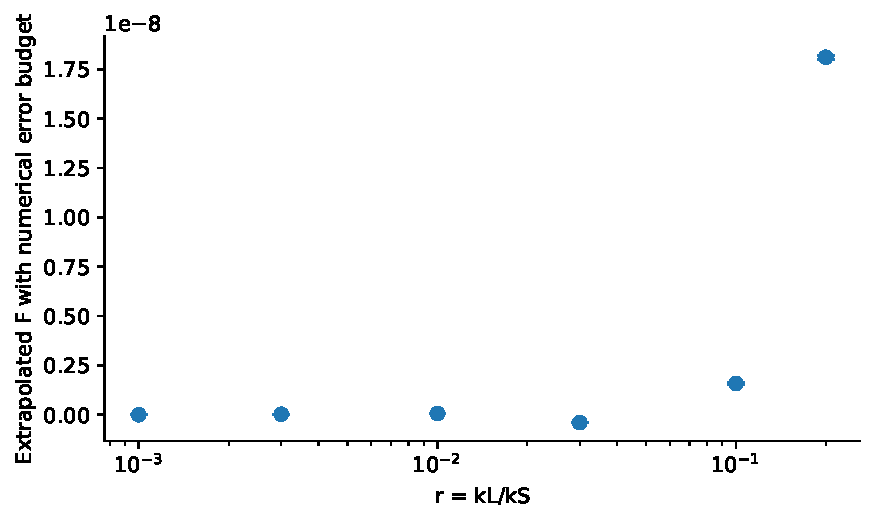
\includegraphics[width=.78\linewidth]{figures/bispectrum_convergence.pdf}\caption{Six pilot triangles with the sum of tested numerical changes. A large relative error near a zero of the oscillation is distinguished from the uncertainty in its envelope.}\end{figure}The largest pilot error normalised to the clock-envelope scale is $0.005845$. This supports a resolved shape scan. Step 9 checks the stronger condition against the fitted oscillatory component itself and tests background and fit-window dependence.
\textbf{Code and supporting data:} \href{https://github.com/rawatpriyansh17/QFT-PROJECT-GROUP-B/tree/main/step8}{step8 on GitHub}.\newpage\section*{Contributions (equal)}\begin{center}\begin{tabularx}{\linewidth}{p{33mm}X}\toprule Member & Contribution\\\midrule Priyansh Rawat & Ultraviolet initial-state derivation and interpretation.\\[3mm]Samarth Bhatnagar & Regulator, cutoff and final-time error budget.\\[3mm]Mayank Sinha & Quadrature/precision comparisons and convergence data.\\\bottomrule\end{tabularx}\end{center}\end{document}